\begin{minipage}{.5\textwidth}
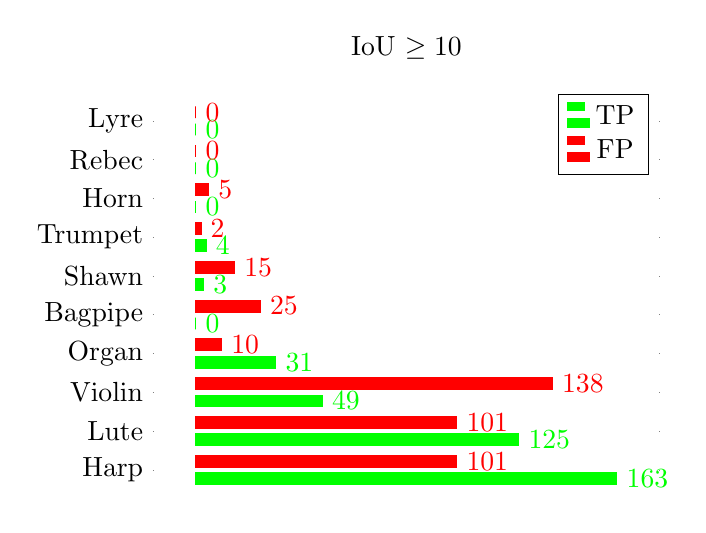
\begin{tikzpicture}
  \begin{axis}[title  = IoU $\geq 10$,
    xbar,
    bar width=.15cm,
    y axis line style = { opacity = 0 },
    axis x line       = none,
    tickwidth         = 0.3pt,
    width=8cm,
    symbolic y coords = {Harp, Lute, Violin, Organ, Bagpipe, Shawn, Trumpet, Horn, Rebec, Lyre},
    ytick= data,
    nodes near coords,
  ]
  \addplot [color=green,fill ] coordinates {(163,Harp) (125,Lute) (49,Violin) (31,Organ) (0,Bagpipe) (3,Shawn) (4,Trumpet) (0,Horn) (0,Rebec) (0,Lyre)};
  \addplot [color=red,fill] coordinates {(101,Harp) (101,Lute) (138,Violin) (10,Organ) (25,Bagpipe) (15,Shawn) (2,Trumpet) (5,Horn) (0,Rebec) (0,Lyre)};
\legend{TP,FP}
\end{axis}
\end{tikzpicture}
 \end{minipage}
 \hspace{3cm}
\begin{minipage}{.5\textwidth}
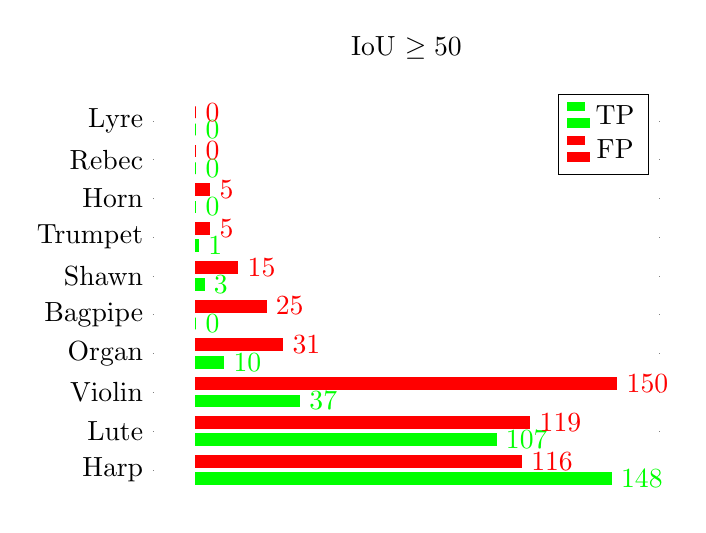
\begin{tikzpicture}
  \begin{axis}[title  = IoU $\geq 50$,
    xbar,
    bar width=.15cm,
    y axis line style = { opacity = 0 },
    axis x line       = none,
    tickwidth         = 0.3pt,
    width=8cm,
    symbolic y coords = {Harp, Lute, Violin, Organ, Bagpipe, Shawn, Trumpet, Horn, Rebec, Lyre},
    ytick=data,
    nodes near coords,
  ]
  \addplot [color=green,fill] coordinates {(148,Harp) (107,Lute) (37,Violin) (10,Organ) (0,Bagpipe) (3,Shawn) (1,Trumpet) (0,Horn) (0,Rebec) (0,Lyre)};
  \addplot [color=red,fill] coordinates {(116,Harp) (119,Lute) (150,Violin) (31,Organ) (25,Bagpipe) (15,Shawn) (5,Trumpet) (5,Horn) (0,Rebec) (0,Lyre)};
\legend{TP,FP}

\end{axis}
\end{tikzpicture}
 \end{minipage}
 

